\def\linkdethi{} %Đường link cần dẫn tới
\anmaQR
%%%%%%%%%%%%%%%%%%%%%%%%
\def\toanlop{12}
\def\thoigian{90}
\def\namhoc{2025 - 2026}
\begin{dethi}
	{Bộ GD\&ĐT}
	{VTED ft KING EDU}
	{TDMZZ02}
	{Đề thi thử THPTQG 2026}
\end{dethi}
\caulc
\Opensolutionfile{ans}[ans/ansTN-Dung]
%%%===============ex_1===============%%%
\begin{ex}%[1D2N3-4]%[TDMZZ02-1-TN]%[Mui Doan]
	Cho cấp số nhân $(u_n)$ có $u_1=1$ và $u_2=2$.
	Giá trị của $u_4$ bằng
	\choice
	{\True $8$}
	{$4$}
	{$16$}
	{$2$}
	\loigiai{
		Công bội $q=\dfrac{u_2}{u_1}=\dfrac{2}{1}=2$.\\
		Ta có $u_4=u_1\cdot q^3=1\cdot 2^3=8$.
	}
\end{ex}

%%%===============ex_2===============%%%
\begin{ex}%[1D6H2-2]%[TDMZZ02]%[Trí Thiện]
	Với hai số thực dương tùy ý $a$ và $b$ thì $\log\left(a^2 \cdot b^5\right)$ bằng
	\choice
	{$10\log a \cdot \log b$}
	{\True $2\log a + 5\log b$}
	{$2\log b + 5\log a$}
	{$5 + \log(a\cdot b)$}
	\loigiai{
		Ta có
		$\log\left(a^2b^5\right) = \log\left(a^2\right) + \log\left(b^5\right) = 2\log a + 5\log b$.
	}
\end{ex}

%%%===============ex_3===============%%%
\begin{ex}%[1D6N3-2]%[TDMZZ02]%[Chu Hà]
	Tập xác định của hàm số $y=\left(x-2\right)^{-2}$ là
	\choice
	{$\left(-\infty;+\infty\right)$}
	{$\left(2;+\infty\right)$}
	{\True $\mathbb{R}\setminus\left\{2\right\}$}
	{$\left[2;+\infty\right)$}
	\loigiai{
		Hàm số $y=\left(x-2\right)^{-2}=\dfrac{1}{\left(x-2\right)^2}$.\\
		Điều kiện xác định là $\left(x-2\right)^2\ne 0 \Leftrightarrow x-2\ne 0 \Leftrightarrow x\ne 2$.\\
		Vậy tập xác định là $\mathscr{D}=\mathbb{R}\setminus\left\{2\right\}$.
	}
\end{ex}

%%%===============ex_4===============%%%
\begin{ex}%[1H8H1-2]%[TDMZZ02]%[Nguyễn Tấn Linh]
	\immini[thm]
	{
		Cho hình lập phương $ABCD.A'B'C'D'$. Đáp án cho nhận xét \textbf{sai} là
		\choice
		{$AA' \perp BD$}
		{$A'C' \perp BD$}
		{$BD \perp A'C$}
		{\True $B'D' \perp C'D$}
	}
	{
		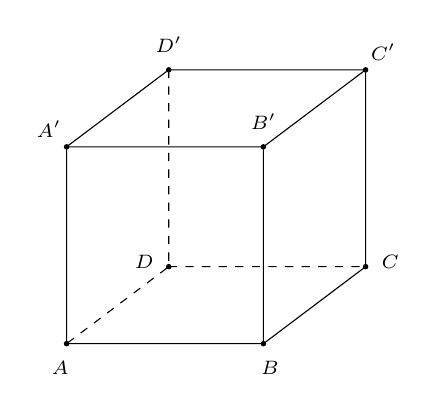
\begin{tikzpicture}[declare function={r=2.5;},font=\scriptsize]
			\path (0:0) coordinate (A)
			(0:r) coordinate (B)
			++(37:{0.65*r}) coordinate (C)
			++(180:r) coordinate (D)
			\foreach \x in {A,B,C,D}{(\x)++(90:r) coordinate (\x_1)};
			\draw[dashed] (D_1)--(D)--(A)
			(D)--(C);
			\draw (A)--(B)--(C)
			(A)--(A_1)
			(B)--(B_1)
			(C)--(C_1)
			(A_1)--(B_1)--(C_1)--(D_1)--cycle;
			\foreach \x/\goc/\t in {A/255/A,B/-75/B,C/10/C,D/170/D,A_1/135/A',B_1/90/B',
				C_1/45/C',D_1/90/D'}{
				\fill (\x) circle (1pt) node[shift={(\goc:9pt)}]{$\t$};
			}
		\end{tikzpicture}
	}
	\loigiai
	{
		\begin{itemize}
			\item Ta có $AA' \perp (ABCD) \Rightarrow AA' \perp BD$.
			\item Ta có $A'C' \parallel AC$ và $AC \perp BD$ (do $ABCD$ là hình vuông) nên $A'C' \perp BD$.
			\item Ta có $\heva{&BD \perp AC \\ &BD \perp AA'} \Rightarrow BD \perp (ACC'A') \Rightarrow BD \perp A'C$.
			\item Ta có $B'D' \parallel BD$. Xét $\triangle BC'D$, ta có $BC'=C'D=BD$ (đều là đường chéo của các hình vuông bằng nhau), suy ra $\triangle BC'D$ là tam giác đều.\\
			Do đó $BD$ không vuông góc với $C'D$, kéo theo $B'D'$ không vuông góc với $C'D$.
		\end{itemize}
	}
\end{ex}

%%%===============ex_5===============%%%
\begin{ex}%[2D1N2-2]%[TDMZZ02]%[Phạm Hải Dương]
	Cho bảng biến thiên của hàm số $f(x)$ như hình vẽ bên dưới. Điểm cực đại của đồ thị hàm số $y = f(x)$ là
	\begin{center}
		\begin{tikzpicture}
			\tkzTabInit[nocadre=false,lgt=1.2,espcl=2.5,deltacl=0.5]
			{$x$/0.75,$f'(x)$/0.75,$f (x)$/3}
			{$-\infty$,$-3$,$0$,$+\infty$}
			\tkzTabLine{,+,0,-,0,+}
			\path
			($(N13)!0.1!(N12)$) node (A1){$ -\infty $}
			($(N23)!0.65!(N22)$) node (A2){$ 2 $}
			($(N33)!0.25!(N32)$) node (A3){$ -1 $}
			($(N43)!0.8!(N42)$) node (A4){$ +\infty $};
			\foreach \x/\y in {A1/A2,A2/A3,A3/A4}{
				\draw[-stealth] (\x)--(\y);
			}
		\end{tikzpicture}
	\end{center}
	\choice
	{\True $(-3; 2)$}
	{$(2; -3)$}
	{$(0; -1)$}
	{$x = -3$}
	\loigiai{
		Dựa vào bảng biến thiên, ta thấy điểm cực đại của đồ thị hàm số $y = f(x)$ là điểm có tọa độ $(-3; 2)$.
	}
\end{ex}

%%%===============ex_6===============%%%
\begin{ex}%[2D1N4-1]%[TDMZZ02]%[Nguyễn Sơn Thành]
	Số đường tiệm cận của đồ thị hàm số $y =\dfrac{1}{x- 1}$ là
	\choice
	{$1$}
	{\True $2$}
	{$3$}
	{$0$}
	\loigiai{
		Ta có
		\begin{itemize}
			\item Tập xác định là $\mathscr{D}=\mathbb{R}\setminus\left\{1\right\}$.
			\item $\displaystyle\lim\limits_{x\to+\infty}\dfrac{1}{x- 1}=0$, $\displaystyle\lim\limits_{x\to-\infty}\dfrac{1}{x-1}=0$ suy ra $y=0$ là tiệm cận ngang của đồ thị hàm số.
			\item $\displaystyle\lim\limits_{x \to \left(1\right)^+} \dfrac{1}{x-1}=+\infty$, $\displaystyle\lim\limits_{x \to \left(1\right)^-} \dfrac{1}{x-1}=-\infty$ suy ra $x=1$ là tiệm cận đứng của đồ thị hàm số.
		\end{itemize}
		Vậy đồ thị hàm số có $2$ đường tiệm cận.
	}
\end{ex}

%%%===============ex_7===============%%%
\begin{ex}%[2D3H2-3]%[TDMZZ02]%[Bồ Văn Hậu]
	Cho hai mẫu số liệu ghép nhóm $M_1$, $M_2$ với bảng tần số ghép nhóm như hình vẽ bên dưới
	\begin{center}
		Nhóm $M_1$
		\begin{tabular}{|c|c|c|c|c|c|c|}
			\hline
			Nhóm & $[8;10)$ & $[10;12)$ & $[12;14)$ & $[14;16)$ & $[16;18)$ & $[18;20)$ \\
			\hline
			Tần số & $6$ & $6$ & $8$ & $4$ & $6$ & $7$ \\
			\hline
		\end{tabular}
	\end{center}
	\begin{center}
		Nhóm $M_2$
		\begin{tabular}{|c|c|c|c|c|c|c|}
			\hline
			Nhóm & $[8;10)$ & $[10;12)$ & $[12;14)$ & $[14;16)$ & $[16;18)$ & $[18;20)$ \\
			\hline
			Tần số & $9$ & $9$ & $12$ & $6$ & $9$ & $n_6$ \\
			\hline
		\end{tabular}
	\end{center}
	Hãy xác định $n_6$ để hai mẫu số liệu trên có độ lệch chuẩn bằng nhau.
	\choice
	{$n_6=10{,}5$}
	{$n_6=7$}
	{$n_6=11$}
	{\True $n_6\in \varnothing$}
	\loigiai{
		Điều kiện: $n_6$ là số tự nhiên.\\
		Giá trị trung bình của mẫu $M_1$ là
		\[\overline{x}_1 = \dfrac{9 \cdot 6 + 11 \cdot 6 + 13 \cdot 8 + 15 \cdot 4 + 17 \cdot 6 + 19 \cdot 7}{6 + 6 + 8 + 4 + 6 + 7}
		= \dfrac{519}{37}.\]
		Phương sai của mẫu $M_1$ là
		\[s_1^2=\dfrac{9^2 \cdot 6 + 11^2 \cdot 6 + 13^2 \cdot 8 + 15^2 \cdot 4 + 17^2 \cdot 6 + 19^2 \cdot 7}{6 + 6 + 8 + 4 + 6 + 7}-\left(\dfrac{519}{37}\right)^2=\dfrac{16\,464}{1\,369}.
		\]
		Giá trị trung bình của mẫu $M_2$ là
		\[\overline{x}_2 = \dfrac{9 \cdot 9 + 11 \cdot 9 + 13 \cdot 12 + 15 \cdot 6 + 17 \cdot 9 + 19 \cdot n_6}{9 + 9 + 12 + 6 + 9 + n_6}
		= \dfrac{579+19n_6}{45+n_6}.\]
		Phương sai của mẫu $M_2$ là
		\[s_2^2=\dfrac{9^2 \cdot 9 + 11^2 \cdot 9 + 13^2 \cdot 12 + 15^2 \cdot 6 + 17^2 \cdot 9 + 19^2 \cdot n_6}{9 + 9 + 12 + 6 + 9 + n_6}-\left(\dfrac{579+19n_6}{45+n_6}\right)^2=\dfrac{7\,797+361n_6}{45+n_6}-\left(\dfrac{579+19n_6}{45+n_6}\right)^2.
		\]
		Hai mẫu số liệu có độ lệch chuẩn bằng nhau thì phương sai tương ứng cũng bằng nhau hay
		\[\dfrac{16\,464}{1\,369}=\dfrac{7\,797+361n_6}{45+n_6}-\left(\dfrac{579+19n_6}{45+n_6}\right)^2 \Rightarrow n_6=10{,}5.\]
		Mà $n_6$ là số tự nhiên nên $n_6=10{,}5$ bị loại hay không có giá trị của $n_6$ thỏa yêu cầu.\\
		\textbf{Cách khác:}\\
		Vì các nhóm của mẫu số liệu $M_1$, $M_2$ hoàn toàn giống nhau nên để hai mẫu số liệu trên có độ lệch chuẩn bằng nhau thì
		\[\dfrac{6}{9}=\dfrac{6}{9}=\dfrac{8}{12}=\dfrac{4}{6}=\dfrac{6}{9}=\dfrac{7}{n_6}\Rightarrow n_6=10{,}5.\]
		Mà $n_6$ là số tự nhiên nên $n_6=10{,}5$ bị loại hay không có giá trị của $n_6$ thỏa yêu cầu.
	}
\end{ex}

%%%===============ex_8===============%%%
\begin{ex}%[2H2H1-2]%[TDMZZ02]%[Lê Phúc]
	\immini[thm]{Cho hình hộp $ABCD.A'B'C'D'$. Phát biểu nào sau đây là đúng?
		\choice
		{$\overrightarrow{AB}+\overrightarrow{B'C}+\overrightarrow{CB'}=\overrightarrow{AB'}$}
		{$\overrightarrow{AC}+\overrightarrow{C'D}+\overrightarrow{DB'}=\overrightarrow{AB'}$}
		{\True $\overrightarrow{AB}+\overrightarrow{CB'}+\overrightarrow{A'D'}=\overrightarrow{AB'}$}
		{$\overrightarrow{AD}+\overrightarrow{DC}+\overrightarrow{C'B'}=\overrightarrow{AB'}$}}
	{
		\begin{tikzpicture}[declare function={a=3; b=0.45*a; h=0.65*a;}]
			\path (0:0) coordinate (A)
			(220:b) coordinate (B)
			($(B)+(a,0)$) coordinate (C)
			(a,0) coordinate (D)
			\foreach \x in {A,B,C,D}{(\x)++(90:h) coordinate (\x1)};
			\draw[dashed] (A1)--(A)--(B)
			(A)--(D);
			\draw (B1)--(A1)--(D1)--(C1)
			(D1)--(D)--(C)
			(B)--(C)--(C1)--(B1)--cycle;
			\foreach \x/\goc/\t in {A/45/A,B/-90/B,C/-90/C,D/0/D,A1/90/A',B1/90/B',C1/90/C',D1/90/D'}
			\fill (\x) circle (1pt) node[shift={(\goc:7pt)},font=\scriptsize]{$\t$};
		\end{tikzpicture}
	}
	\loigiai{
		\begin{itemize}
			\item
			$\overrightarrow{AB}+\overrightarrow{B'C}+\overrightarrow{CB'}=\overrightarrow{AB'}
			\Leftrightarrow\overrightarrow{0}=\overrightarrow{AB'}-\overrightarrow{AB}
			\Leftrightarrow\overrightarrow{0}=\overrightarrow{BB'}$ (sai).
			\item
			$\overrightarrow{AC}+\overrightarrow{C'D}+\overrightarrow{DB'}=\overrightarrow{AB'}		\Leftrightarrow\overrightarrow{A'C'}+\overrightarrow{C'D}=\overrightarrow{AB'}-\overrightarrow{DB'}
			\Leftrightarrow\overrightarrow{A'D}=\overrightarrow{AD}$ (sai).
			\item
			$\overrightarrow{AB}+\overrightarrow{CB'}+\overrightarrow{A'D'}=\overrightarrow{AB'}
			\Leftrightarrow \overrightarrow{CB'}+\overrightarrow{B'C'}=\overrightarrow{AB'}-\overrightarrow{AB}
			\Leftrightarrow\overrightarrow{CC'}=\overrightarrow{BB'}$ (đúng).
			\item
			$\overrightarrow{AD}+\overrightarrow{DC}+\overrightarrow{C'B'}=\overrightarrow{AB'}
			\Leftrightarrow \overrightarrow{AC}=\overrightarrow{AB'}-\overrightarrow{C'B'}
			\Leftrightarrow\overrightarrow{AC}=\overrightarrow{AC'}$ (sai).
		\end{itemize}
	}
\end{ex}

%%%===============ex_9===============%%%
\begin{ex}%[2D4H2-4]%[TDMZZ02]%[Trần Văn Thiện]
	Nếu $C$ là một hắng số thực thì họ nguyên hàm của hàm số $f(x)=2^x\ln 2+\dfrac{1}{x}$ là
	\choice
	{$F(x)=2^x+\ln x +C^2$}
	{$F(x)=2^x\ln 2+\ln|x|+C$}
	{\True $F(x)=2^x+\ln|x|+C+2\,026$}
	{$F(x)=2^x+\ln|x|+|C|$}
	\loigiai{
		Ta có $F(x)=\displaystyle\int f(x)\mathrm{\,d}x=\displaystyle\int \left(2^x\ln 2+\dfrac{1}{x}\right)\mathrm{\,d}x=2^x+\ln|x|+C'$ ($C'$ là hằng số thực).\\
		Thay $C'=C+2\,026$ ta có $\displaystyle\int f(x)\mathrm{\,d}x=2^x+\ln|x|+C+2\,026$.
	}
\end{ex}

%%%===============ex_10===============%%%
\begin{ex}%[2D4H2-1]%[TDMZZ02]%[Đình Nguyên]
	Nếu $\displaystyle\int\limits_1^0 f(x)\mathrm{\,d}x = 2$ và $\displaystyle\int\limits_1^2 f(x)\mathrm{\,d}x = 3$ thì $\displaystyle\int\limits_0^2 f(x)\mathrm{\,d}x$ bằng
	\choice
	{\True $1$}
	{$5$}
	{$6$}
	{$0$}
	\loigiai{
		Ta có $\displaystyle\int\limits_0^1 f(x)\mathrm{\,d}x = -\int\limits_1^0 f(x)\mathrm{\,d}x = -2$.\\
		Khi đó $\displaystyle\int\limits_0^2 f(x)\mathrm{\,d}x = \int\limits_0^1 f(x)\mathrm{\,d}x + \int\limits_1^2 f(x)\mathrm{\,d}x = -2 + 3 = 1$.
	}
\end{ex}

%%%===============ex_11===============%%%
\begin{ex}%[2H2N2-4]%[TDMZZ02]%[Huỳnh Quốc Đạt]
	Trong không gian $Oxyz$, cho điểm $A(1;2;-2)$ và điểm $B(3;0;2)$. Độ dài đoạn thẳng $AB$ bằng
	\choice
	{$2\sqrt{3}$}
	{\True $2\sqrt{6}$}
	{$4$}
	{$3\sqrt{6}$}
	\loigiai{Ta có $\overrightarrow{AB}=(2;-2;4)$. Khi đó $AB=\sqrt{2^2+(-2)^2+4^2}=2\sqrt{6}$.}
\end{ex}

%%%===============ex_12===============%%%
\begin{ex}%[2H5N3-2]%[TDMZZ02]%[Nguyễn Trí Minh Tuấn]
	Trong không gian $Oxyz$, tọa độ tâm của mặt cầu
	$(S)\colon 3x^2+3y^2+3z^2-12x=0$
	là
	\choice
	{$(6;0;0)$}
	{$(0;2;0)$}
	{$(3;2;0)$}
	{\True $(2;0;0)$}
	\loigiai{
		Ta có
		\[
		3x^2+3y^2+3z^2-12x=0 \Leftrightarrow
		x^2+y^2+z^2-4x=0
		\Leftrightarrow
		(x-2)^2+y^2+z^2=4.
		\]
	}
\end{ex}
\Closesolutionfile{ans}


\cauds
\Opensolutionfile{ans}[ans/ansTN-DungSai]
%%%===============extf_1===============%%%
\begin{ex}%[2D4H3-1]%[TDMZZ02]%[Văn Minh Thoại]
	Cho hàm số $y=f(x)=\dfrac{x+3}{x-1}$ có đồ thị $(C)$.
	\choiceTF
	{\True Tập xác định của hàm số $f(x)$ là $(-\infty;1)\cup(1;+\infty)$}
	{Hàm số $f(x)$ nghịch biến trên tập xác định của nó}
	{\True Đồ thị $(C)$ có tâm đối xứng là $I(1;1)$}
	{\True Diện tích hình phẳng giới hạn bởi $(C)$ và hai trục toạ độ là $2{,}55$ \textit{(làm tròn kết quả đến hàng phần trăm)}}
	\loigiai{
		\begin{itemchoice}
			\itemch Hàm số $y=f(x)=\dfrac{x+3}{x-1}$ xác định khi $x-1\neq0\Leftrightarrow x\neq1$.\\
			Tập xác định của hàm số $f(x)$ là $\mathscr{D}=(-\infty;1)\cup(1;+\infty)$.
			\itemch Ta có $y=f(x)=\dfrac{x+3}{x-1}$.\\
			Suy ra $f'(x)=\dfrac{1\cdot(-1)-3\cdot1}{(x-1)^2}=\dfrac{-4}{(x-1)^2}<0$, $\forall x\neq1$.\\
			Hàm số nghịch biến trên từng khoảng $(-\infty;1)$ và $(1;+\infty)$.\\
			Hàm số không nghịch biến trên tập xác định $\mathscr{D}$ của nó.
			\itemch Đồ thị hàm số có đường tiệm cận đứng $x=1$ và đường tiệm cận ngang $y=1$.\\
			Tâm đối xứng của đồ thị là giao điểm của hai đường tiệm cận, suy ra đồ thị $(C)$ có tâm đối xứng là $I(1;1)$.
			\itemch Đồ thị $(C)$ cắt trục hoành tại điểm có tọa độ $(-3;0)$.\\
			Đồ thị $(C)$ cắt trục tung tại điểm có tọa độ $(0;-3)$.\\
			Diện tích hình phẳng giới hạn bởi $(C)$ và hai trục toạ độ $Ox$ (có phương trình $y=0$), $Oy$ (có phương trình $x=0$) là
			\allowdisplaybreaks
			\begin{eqnarray*}
				S&=&\displaystyle\int\limits_{-3}^{0}\left|\dfrac{x+3}{x-1}\right|\mathrm{\,d}x	\\
				&=&\displaystyle\int\limits_{-3}^{0}\dfrac{-(x+3)}{x-1}\mathrm{d}x \quad(\text{do } x\in[-3;0] \text{ thì } \dfrac{x+3}{x-1}\leq0)\\
				&=&\displaystyle\int\limits_{-3}^{0}\left(-1-\dfrac{4}{x-1}\right)\mathrm{d}x\\
				&=&\left(-x-4\ln|x-1|\right)\Big|_{-3}^{0}\\
				&=&(0-4\ln1)-(3-4\ln|-4|)\\
				&=&-3+4\ln4\\
				&\approx&2{,}55.
			\end{eqnarray*}
		\end{itemchoice}
	}
\end{ex}

%%%===============extf_2===============%%%
\begin{ex}%[2D4V3-3]%[TDMZZ02]%[Dương Công Tạo]
	Cho hàm số $y=f(x)=k\sqrt{x}$ ($k>0$) có đồ thị là một nửa đường parabol $(P)$. Xét hình phẳng $(H)$ giới hạn bởi $(P)$, $y = 0$ và đường thẳng $x=h$ ($h>0$), gọi điểm $M(h;R)\in (P)$.
	\choiceTF
	{\True $R=k\sqrt{h}$}
	{\True Diện tích hình phẳng $(H)$ bằng $\dfrac{2}{3} Rh$}
	{\True Thể tích khối tròn xoay thu được khi cho $(H)$ quay quanh $Ox$ là $\dfrac{\pi}{2} R^2h$}
	{\True Thể tích khối tròn xoay thu được khi cho hình phẳng giới hạn bởi $y = R$; $y = 0$; $x = 0$; $x = h$ quay quanh $Ox$ gấp đôi khi cho $(H)$ quay quanh $Ox$}
	\loigiai{
		\begin{itemchoice}
			\itemch Ta có $M(h;R)\in (P)\Leftrightarrow R=k\sqrt{h}$.
			\itemch Diện tích hình phẳng $(H)$ là $S=\displaystyle\int\limits_0^h{k\sqrt{x}}\mathrm{\,d}x=\dfrac{2k}{3}\big.\sqrt{x^3}\Bigg|_0^h=\dfrac{2k}{3}\sqrt{h^3}=\dfrac{2}{3}h\cdot k\sqrt{h}$.\\
			Mà $R=k\sqrt{h}$ nên $S=\dfrac{2}{3}Rh$.
			\itemch Thể tích khối tròn xoay thu được khi cho $(H)$ quay quanh $Ox$ là \[V=\pi\displaystyle\int\limits_0^h\left(k\sqrt{x}\right)^2\mathrm{\,d}x=k^2\pi\displaystyle\int\limits_0^h{x}\mathrm{\,d}x=k^2\dfrac{\pi}{2}\big.x^2\bigg|_0^h=\dfrac{\pi}{2}k^2h^2.\]
			Mà $R=k\sqrt{h}$ nên $k^2=\dfrac{R^2}{h}$.\\
			Khi đó $V=\dfrac{\pi}{2}h^2\cdot\dfrac{R^2}{h}=\dfrac{\pi}{2}R^2h$.
			\itemch Hình phẳng giới hạn bởi $y = R$; $y = 0$; $x = 0$; $x = h$ là hình chữ nhật nên khi quay quanh $Ox$ ta thu được một hình trụ có thể tích là $V_1=\pi R^2h=2V$.
		\end{itemchoice}
	}
\end{ex}

%%%===============extf_3===============%%%
\begin{ex}%[2H5V2-8]%[TDMZZ02]%[Nguyễn Văn Sang]
	\immini[thm]{Trong không gian $Oxyz$, có một gương cầu lõm có dạng một chỏm cầu $(G)$ có tâm $O$ và bán kính $R>0$ phản xạ mọi tia sáng chiếu tới nó. Một tia sáng xuất phát từ nguồn sáng điểm $S(2;0;1)$ đến gặp mặt gương $(G)$ tại điểm $K(2;-4;4)$, tại $K$ tia sáng bị bật ngược trở lại đi qua điểm $T$, sao cho: $T \in (SKO)$, $\widehat{SKO} = \widehat{OKT}$.
		\choiceTF
		{\True $\left(\overrightarrow{KS},\overrightarrow{KO}\right)=21^\circ$ \textit{(làm tròn kết quả đến hàng đơn vị)}}
		{\True Phương trình tham số của đường thẳng $SK$ là $\heva{& x = 2 \\ & y = 4t \\ & z = 1 - 3t.}$}
		{\True Bán kính của gương $R = 6$}
		{Tia phản xạ $KT$ cắt mặt phẳng $(Oxy)$ tại điểm có hoành độ bằng $2$}
	}
	{\begin{tikzpicture}[>=stealth,scale=0.8,line join=round,line cap=round]
			% Points for reflection
			\coordinate (O2) at (3,1);
			\coordinate (S) at (4,-1);
			\coordinate (K) at (7,2.5);
			\coordinate (T) at (2,3.5);
			% Drawn elements
			\draw[blue] (6.5,-0.5) to[bend right=20] (K) to[bend right=15] (5.5,5);
			\draw[->,red] (S) -- ($(S)!0.6!(K)$);
			\draw[red] ($(S)!0.6!(K)$) -- (K);
			\draw[->,red] (K) -- ($(K)!0.6!(T)$);
			\draw[red] ($(K)!0.6!(T)$) -- (T);
			\draw (O2) -- (K);
			\fill (O2) circle (1.5pt) node[below]{$O$};
			\fill (S) circle (1.5pt) node[below]{$S$};
			\fill (K) circle (1.5pt) node[right]{$K$};
			\node[above] at (T) {$T$};
		\end{tikzpicture}
	}
	\loigiai{
		Ta có $S(2;0;1)$, $K(2;-4;4)$ và $O(0;0;0)$. Suy ra $\overrightarrow{KS} = (0;4;-3)$ và $\overrightarrow{KO} = (-2;4;-4)$.
		\begin{itemchoice}
			\itemch $\cos\left(\overrightarrow{KS},\overrightarrow{KO}\right) = \dfrac{\overrightarrow{KS}\cdot\overrightarrow{KO}}{\left|\overrightarrow{KS}\right| \cdot \left|\overrightarrow{KO}\right|} = \dfrac{0\cdot(-2) + 4\cdot 4 + (-3)\cdot(-4)}{\sqrt{0^2+4^2+(-3)^2}\cdot\sqrt{(-2)^2+4^2+(-4)^2}} = \dfrac{28}{5\cdot 6} = \dfrac{14}{15}$.\\
			Suy ra $\left(\overrightarrow{KS},\overrightarrow{KO}\right) \approx 21^\circ$.
			\itemch Đường thẳng $SK$ đi qua điểm $S(2;0;1)$ và nhận $\overrightarrow{KS} = (0;4;-3)$ làm vectơ chỉ phương.\\
			Nên phương trình tham số của nó là: $\heva{& x = 2 \\ & y = 4t \\ & z = 1 - 3t .}$
			\itemch Do điểm $K(2;-4;4)$ nằm trên gương cầu tâm $O(0;0;0)$ nên bán kính gương là $$R = OK = \sqrt{2^2+(-4)^2+4^2} = 6.$$
			\itemch Tia phản xạ $KT$ và tia tới $KS$ đối xứng nhau qua pháp tuyến $KO$, hay nói cách khác đường thẳng $KO$ là phân giác của góc $\widehat{SKT}$.
			\immini
			{Gọi $S'$ là điểm đối xứng của $S$ qua đường thẳng $KO$, khi đó $S'$ nằm trên đường thẳng chứa tia phản xạ $KT$.\\
				Đường thẳng $KO$ đi qua $O(0;0;0)$ và có vectơ chỉ phương\\ $\overrightarrow{u} = -\dfrac{1}{2}\overrightarrow{KO} = (1;-2;2)$ nên có phương trình tham số: $\heva{& x = m \\ & y = -2m \\ & z = 2m.}$
			}{	
			\begin{tikzpicture}[>=stealth,scale=0.8,line join=round,line cap=round]
				\coordinate (O2) at (3,1);
				\coordinate (S) at (4,-1);
				\coordinate (K) at (7,2.5);
				\coordinate (T) at (2,3.5); % Original T direction
				\coordinate (H) at ($(O2)!(S)!(K)$); % Projection of S on OK
				\coordinate (S') at ($(S)!2!(H)$); % Reflection of S across OK
				\draw[blue] (6.5,-0.5) to[bend right=20] (K) to[bend right=15] (5.5,5);
				\draw[->,red] (S) -- ($(S)!0.5!(K)$);
				\draw[red] ($(S)!0.5!(K)$) -- (K);
				\draw[->,red] (K) -- ($(K)!0.5!(S')$);
				\draw[red] ($(K)!0.5!(S')$) -- (S');
				\draw[dashed] (O2) -- (K);
				\draw[gray,dashed] (S) -- (S');
				\draw[gray,dashed] (K) -- (S') node[midway,sloped,allow upside down]{\tiny{$/\!/$}};
				\draw[gray,dashed] (K) -- (S) node[midway,sloped,allow upside down]{\tiny{$/\!/$}};
				\fill (O2) circle (1.5pt) node[below left]{$O$};
				\fill (S) circle (1.5pt) node[below right]{$S$};
				\fill (K) circle (1.5pt) node[right]{$K$};
				\fill (H) circle (1.5pt) node[below right]{$H$};
				\fill (S') circle (1.5pt) node[above left]{$S'$};
				\node[above right] at (S') {$T$};
				\foreach \x/\y/\z in {S/H/O2}{
					\path (\y) pic[draw,angle radius=5pt]{right angle = \x--\y--\z};
				}
			\end{tikzpicture}
			}
			\noindent
			Gọi $H(m; -2m; 2m)$ là hình chiếu vuông góc của $S$ lên $KO$. Ta có $\overrightarrow{SH} = (m-2; -2m; 2m-1)$.\\
			Vì $SH \perp KO$ nên $\overrightarrow{SH} \cdot \overrightarrow{u} = 0 \Leftrightarrow 1(m-2) - 2(-2m) + 2(2m-1) = 0 \Leftrightarrow 9m - 4 = 0 \Leftrightarrow m = \dfrac{4}{9}$.\\
			Suy ra $H\left(\dfrac{4}{9}; -\dfrac{8}{9}; \dfrac{8}{9}\right)$. Vì $H$ là trung điểm của $SS'$ nên $S'\left(-\dfrac{10}{9}; -\dfrac{16}{9}; \dfrac{7}{9}\right)$.\\
			Đường thẳng chứa tia phản xạ $KT$ đi qua $K(2;-4;4)$ và $S'\left(-\dfrac{10}{9}; -\dfrac{16}{9}; \dfrac{7}{9}\right)$, suy ra vectơ chỉ phương $\overrightarrow{KS'} = \left(-\dfrac{28}{9}; \dfrac{20}{9}; -\dfrac{29}{9}\right)$.\\
			Chọn vectơ chỉ phương của tia $KT$ là $\overrightarrow{v} = 9\overrightarrow{KS'} = (-28;20;-29)$.\\
			Phương trình tham số của tia $KT$ là $\heva{& x = 2 - 28t \\ & y = -4 + 20t \\ & z = 4 - 29t .}$\\
			Tia $KT$ cắt mặt phẳng $(Oxy)$ (có phương trình $z=0$) khi $4 - 29t = 0 \Leftrightarrow t = \dfrac{4}{29}$.\\
			Thay $t=\dfrac{4}{29}$ vào $x$, ta được hoành độ giao điểm là $x = 2 - 28\cdot\dfrac{4}{29} = -\dfrac{54}{29} \approx -1{,}86 \neq 2$.
		\end{itemchoice}
	}
\end{ex}

%%%===============extf_4===============%%%
\begin{ex}%[2D6V2-4]%[TDMZZ02]%[Vũ Hồng Toàn]
	Một công ty có sản xuất một loại sản phẩm. Trước khi bán ra thị trường thì có phỏng vấn $200$ khách hàng và thấy có $90$ người trả lời \lq\lq sẽ mua\rq\rq, $50$ người trả lời \lq\lq không mua\rq\rq~còn lại trả lời \lq\lq sẽ cân nhắc\rq\rq~thêm và hiện tại chưa quyết định sẽ mua hay không mua. Theo thống kê bằng các đợt bán các sản phẩm trước thì trong những khách hàng trả lời sẽ mua thì sẽ có $80\%$ là thực sự mua, trong những khách hàng trả lời không mua thì sẽ có $30\%$ thực sự mua và có $65\%$ tổng số người phỏng vấn là thực sự mua. Chọn ngẫu nhiên một khách hàng trong các khách hàng đã được phỏng vấn.
	\choiceTF
	{\True Xác suất để chọn được người trả lời sẽ mua là $45\%$}
	{Xác suất để chọn được khách hàng thực sự mua, nếu đã biết khách hàng này đã trả lời \lq\lq sẽ mua\rq\rq, là $36\%$}
	{\True Nếu chọn được khách hàng trả lời \lq\lq sẽ cân nhắc\rq\rq~thì tỉ lệ thực sự mua là $\dfrac{43}{60}$}
	{\True Xác suất để chọn được khách hàng trả lời \lq\lq sẽ cân nhắc\rq\rq, nếu biết khách hàng đó thực sự mua là $\dfrac{43}{130}$}
	\loigiai{
		Gọi $A_1$ là biến cố \lq\lq Khách hàng trả lời sẽ mua\rq\rq.\\
		Gọi $A_2$ là biến cố \lq\lq Khách hàng trả lời không mua\rq\rq.\\
		Gọi $A_3$ là biến cố \lq\lq Khách hàng trả lời sẽ cân nhắc\rq\rq.\\
		Gọi $B$ là biến cố \lq\lq Khách hàng thực sự mua\rq\rq.\\
		Dựa vào đề bài, ta có:
		\begin{itemize}
			\item $\mathrm{P}(A_1) = \dfrac{90}{200} = 0{,}45$.
			\item $\mathrm{P}(A_2) = \dfrac{50}{200} = 0{,}25$.
			\item $\mathrm{P}(A_3) = \dfrac{200 - (90 + 50)}{200} = 0{,}3$.
			\item $\mathrm{P}(B\mid A_1) = 80\% = 0{,}8$.
			\item $\mathrm{P}(B\mid A_2) = 30\% = 0{,}3$.
			\item $\mathrm{P}(B) = 65\% = 0{,}65$.
		\end{itemize}
		\begin{itemchoice}
			\itemch Vì $\mathrm{P}(A_1) = 0{,}45 = 45\%$.
			\itemch Xác suất để chọn được khách hàng thực sự mua, nếu đã biết khách hàng này đã trả lời \lq\lq sẽ mua\rq\rq\ là xác suất có điều kiện $\mathrm{P}(B\mid A_1)$.\\
			Theo giả thiết, $\mathrm{P}(B\mid A_1) = 80\% = 0{,}8 \ne 36\%$.\\
			\textit{(Lưu ý: $36\%$ là xác suất chọn được khách hàng trả lời \lq\lq sẽ mua\rq\rq\ và thực sự mua $\mathrm{P}(A_1 \cap B) = \mathrm{P}(A_1) \cdot \mathrm{P}(B \mid A_1) = 0{,}45 \cdot 0{,}8 = 0{,}36 = 36\%$).}
			\itemch Tỉ lệ thực sự mua trong số những khách hàng trả lời \lq\lq sẽ cân nhắc\rq\rq\ là $\mathrm{P}(B\mid A_3)$.\\
			Áp dụng công thức xác suất toàn phần, ta có
			\allowdisplaybreaks
			\begin{align*}
				\mathrm{P}(B) &= \mathrm{P}(A_1) \cdot \mathrm{P}(B\mid A_1) + \mathrm{P}(A_2) \cdot \mathrm{P}(B\mid A_2) + \mathrm{P}(A_3) \cdot \mathrm{P}(B\mid A_3)\\
				\Rightarrow 0{,}65 &= 0{,}45 \cdot 0{,}8 + 0{,}25 \cdot 0{,}3 + 0{,}3 \cdot \mathrm{P}(B\mid A_3)\\
				\Rightarrow 0{,}65 &= 0{,}36 + 0{,}075 + 0{,}3 \cdot \mathrm{P}(B\mid A_3)\\
				\Rightarrow 0{,}3 \cdot \mathrm{P}(B\mid A_3) &= 0{,}215\\
				\Rightarrow \mathrm{P}(B\mid A_3) &= \dfrac{0{,}215}{0{,}3} = \dfrac{43}{60}.
			\end{align*}
			\itemch Xác suất để chọn được khách hàng trả lời \lq\lq sẽ cân nhắc\rq\rq, nếu biết khách hàng đó thực sự mua là $\mathrm{P}(A_3\mid B)$.\\
			Áp dụng công thức Bayes, ta có
			\[
			\mathrm{P}(A_3\mid B) = \dfrac{\mathrm{P}(A_3) \cdot \mathrm{P}(B\mid A_3)}{\mathrm{P}(B)}
			=\dfrac{0{,}215}{0{,}65} = \dfrac{43}{130}.
			\]
		\end{itemchoice}
	}
\end{ex}
\Closesolutionfile{ans}


\caukq
\Opensolutionfile{ans}[ans/ansTN-DienKhuyet]
%%%===============tln_1===============%%%
\begin{ex}%[1H8V7-3]%[TDMZZ02]%[Võ Hiệp]
	Cho hình chóp $S.ABCD$ có đáy $ABCD$ là hình vuông có cạnh bằng $6$, cạnh bên $SA$ vuông góc với đáy. Biết $\mathrm{d}\big(A,(SBC)\big)=\dfrac{\sqrt{5}}{2}\mathrm{d}\big(A,(SBD)\big)$. Hãy tính thể tích của hình chóp $S.ABCD$ ({\it làm tròn kết quả đến hàng phần mười}).
	\par
	\shortans[0]{41,6}
	\loigiai{
		\begin{center}
			\begin{tikzpicture}[scale=1,font=\footnotesize,line join=round,line cap=round,>=stealth]
				\def\a{4}
				\def\h{4}
				\path (0:0) coordinate (A)
				++(0:\a) coordinate (B)
				++(-130:\a/2) coordinate (C)
				($(A)+(C)-(B)$) coordinate (D)
				($(A)+(90:\h)$) coordinate (S)
				(intersection of A--C and B--D) coordinate (O)
				($(S)!.5!(B)$) coordinate (K)
				($(S)!.7!(O)$) coordinate (H); %giao điểm O
				\draw[dashed](B)--(A)--(D)
				(A)--(S)--(O)
				(B)--(D)
				(A)--(C)
				(A)--(K)
				(A)--(H);
				\draw (B)-- (C)--(D)
				(B)--(S)
				(C)--(S)
				(D)--(S);
				\foreach \x/\g in {A/135,B/45,C/-45,D/-135,S/90,O/-90,H/0,K/30}
				\fill (\x) circle (1.5pt)
				($(\g:3mm)+(\x)$) node {$\x$};
				\draw pic[draw,angle radius=2mm]{right angle=A--H--O};
				\draw pic[draw,angle radius=2mm]{right angle=A--K--B};
			\end{tikzpicture}
		\end{center}
		Gọi $O$ là giao điểm của $AC$ và $BD$.
		Gọi $H$ là hình chiếu vuông góc của $A$ trên $SO$. Khi đó ta có
		\begin{itemize}
			\item $\heva{&BD\perp AC ~ (\text{vì}\,\, ABCD \, \text{ là hình vuông})\\
				&BD\perp SA ~ (\text{vì}\,\, SA\perp (ABCD))}\Rightarrow BD\perp (SAO)\Rightarrow BD\perp AH\subset (SAO)$.
			\item $\heva{&AH\perp BD\\
				&AH\perp SO}\Rightarrow AH\perp (SBD)\Rightarrow AH=\mathrm{d}\big(A,(SBD)\big)$.
		\end{itemize}
		Gọi $K$ là hình chiếu vuông góc của $A$ trên $SB$. Khi đó ta có
		\begin{itemize}
			\item $\heva{&BC\perp AB ~ (\text{vì}\,\, ABCD \, \text{ là hình vuông})\\
				&BC\perp SA ~ (\text{vì}\,\, SA\perp (ABCD))}\Rightarrow BC\perp (SAB)\Rightarrow BC\perp AK\subset (SAB)$.
			\item $\heva{&AK\perp BC\\
				&AK\perp SB}\Rightarrow AK\perp (SBC)\Rightarrow AK=\mathrm{d}\big(A,(SBC)\big)$.
		\end{itemize}
		Ta có $ABCD$ là hình vuông có cạnh bằng $6$, suy ra $AO=\dfrac{AC}{2} =\dfrac{6\sqrt{2}}{2}=3\sqrt{2}$. Đặt $SA =x$ ($x>0$).\\
		Áp dụng hệ thức lượng trong các tam giác $\triangle SAO$ và $\triangle SAB$ vuông tại $A$. Ta có
		\begin{itemize}
			\item $\dfrac{1}{AH^2} = \dfrac{1}{SA^2} + \dfrac{1}{AO^2}\Rightarrow
			AH=\dfrac{SA\cdot AO}{\sqrt{SA^2+ AO^2}}=\dfrac{3\sqrt{2} \cdot x}{\sqrt{x^2+18}}$.
			\item $\dfrac{1}{AK^2} = \dfrac{1}{SA^2} + \dfrac{1}{AB^2}\Rightarrow
			AK=\dfrac{SA\cdot AB}{\sqrt{SA^2+ AB^2}}=\dfrac{6x}{\sqrt{x^2+ 36}}$.
		\end{itemize}
		Theo đề bài ta có
		\allowdisplaybreaks
		\begin{eqnarray*}
			\mathrm{d}\big(A,(SBC)\big)=\dfrac{\sqrt{5}}{2}\mathrm{d}\big(A,(SBD)\big)
			&\Rightarrow& AK = \dfrac{\sqrt{5}}{2}AH\\
			&\Rightarrow&\dfrac{6x}{\sqrt{x^2+ 36}}=\dfrac{\sqrt{5}}{2}\cdot \dfrac{3\sqrt{2} \cdot x}{\sqrt{x^2+18}}\\
			&\Rightarrow& \dfrac{36x^2}{x^2+ 36}= \dfrac{90x^2}{4(x^2+18)}\\
			&\Rightarrow& 72(x^2+18)=45(x^2+36)\\
			&\Rightarrow& 27 x^2= 324\\
			&\Rightarrow& x= 2\sqrt{3} \quad (\text{do} \,\, x>0).\\
		\end{eqnarray*}
		Thể tích khối chóp $S.ABCD$ là
		\[V = \dfrac{1}{3} \cdot S_{ABCD} \cdot SA= \dfrac{1}{3} \cdot 36 \cdot 2\sqrt{3} =24\sqrt{3}\approx 41{,}6.\]
	}
\end{ex}

%%%===============tln_2===============%%%
\begin{ex}%[2D4V3-1]%[TDMZZ02]%[Lương Pho]
	\immini[thm]{Cho một mặt bàn hình vuông $ABCD$ có cạnh bằng $120$ cm.
		Để tạo thành một mặt bàn đẹp người ta vát ở bốn góc bởi những phần parabol bằng nhau sao cho đỉnh của parabol cách tâm của mặt bàn $78$ cm và parabol tiếp xúc với hai cạnh của hình vuông ở mỗi góc bàn.
		Hãy tính diện tích mặt bàn sau khi đã vát theo đơn vị mét vuông (\textit{làm tròn kết quả đến hàng phần trăm}).}{
		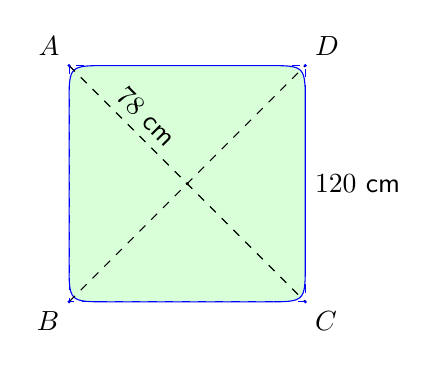
\begin{tikzpicture}[scale=.3,font=\sffamily]
			\def\R{60/12} % Nửa cạnh hình vuông (60cm)
			\def\yt{40.612/12}
			\coordinate (A) at (-\R,\R);
			\coordinate (B) at (-\R,-\R);
			\coordinate (C) at (\R,-\R);
			\coordinate (D) at (\R,\R);
			\coordinate (A1) at (-\yt,\R);
			\coordinate (A2) at (-\R,\yt);
			\coordinate (B1) at (-\R,-\yt);
			\coordinate (B2) at (-\yt,-\R);
			\coordinate (C1) at (\yt,-\R);
			\coordinate (C2) at (\R,-\yt);
			\coordinate (D1) at (\R,\yt);
			\coordinate (D2) at (\yt,\R);
			\fill[fill=green!15]
			(A1).. controls (A).. (A2) --
			(B1).. controls (B).. (B2) --
			(C1).. controls (C).. (C2) --
			(D1).. controls (D).. (D2) -- cycle;
			\draw[blue]
			(A1).. controls (A).. (A2) --
			(B1).. controls (B).. (B2) --
			(C1).. controls (C).. (C2) --
			(D1).. controls (D).. (D2) -- cycle;
			\draw[dashed,blue] (A) -- (B) -- (C) -- (D) -- cycle;
			\draw[dashed,thin] (A) -- (C);
			\draw[dashed,thin] (B) -- (D);
			\fill (0,0) circle (.07); % Tâm bàn
			\fill[blue] (A) circle (.07);
			\fill[blue] (B) circle (.07);
			\fill[blue] (C) circle (.07);
			\fill[blue] (D) circle (.07);
			\node[above left] at (A) {$A$};
			\node[below left] at (B) {$B$};
			\node[below right] at (C) {$C$};
			\node[above right] at (D) {$D$};
			\node[right] at (\R,0) {$120$ cm};
			\coordinate (VA) at ({-39*sqrt (2)/12},{39*sqrt (2)/12});
			\path (0,0) -- (VA) node[midway,sloped,above] {$78$ cm};
		\end{tikzpicture}
	}
	\par
	\shortans[0]{1,41}
	\loigiai{
		\begin{center}
			\begin{tikzpicture}[line cap=round,line join=round,>=stealth,scale=1,font=\footnotesize,declare function={
					xmin=-2.5; xmax=7;
					ymin=-0.5; ymax=7; a=-0.25;
					f (\x)=a*(\x)^2+5;
				},scale=0.8]\draw[->] (xmin,0)--(xmax,0) node[shift={(-100:7pt)}]{$x$};
				\draw[->] (0,ymin)--(0,ymax) node[shift={(0:7pt)}]{$y$};
				\fill (0,0) node[shift={(225:9pt)}]{$O$};
				\clip (xmin,ymin) rectangle (xmax,ymax);
				\draw[smooth,samples=300] plot[domain=-2:2] (\x,{f (\x)});
				\draw (-2,4)--(0,6)--(2,4);
				\draw[dashed] (2,0)--(2,4)
				(-2,0)--(-2,4);
				\draw (0,6)--(6,0) node[shift={(-90:9pt)}]{$D$};
				\foreach \y/\nhan in {5/78,6/A}{
					\fill (0,\y) circle (1pt) node[shift={(45:9pt)}]{$\nhan$};}
			\end{tikzpicture}
		\end{center}
		Ta có $OA=OD=60\sqrt{2}$ nên ta có phương trình $AD$ là \[AD\colon \dfrac{x}{60\sqrt{2}}+\dfrac{y}{60\sqrt{2}}=1\Leftrightarrow y=-x+60\sqrt{2}.\]
		Phương trình parabol $(P)$ có đỉnh $I(0;78)$ nên có dạng $(P)\colon y=ax^2+78$.\\
		Parabol $(P)$ tiếp xúc đường thẳng $AD$ nên
		\[ax^2+78=-x+60\sqrt{2}\Leftrightarrow ax^2+x+78-60\sqrt{2}=0 \text{ có nghiệm kép.}\]
		Do đó $\Delta=1^2-4\cdot a\cdot \left(78-60\sqrt{2}\right)=0\Leftrightarrow a=\dfrac{1}{4\left(78-60\sqrt{2}\right)}$.\\
		Khi đó, parabol $(P)$ tiếp xúc đường thẳng $AD$ tại điểm có hoành độ $x_0=\dfrac{-1}{2a}$.\\
		Suy ra diện tích mặt bàn sau khi đã vát là
		\[120^2-8\displaystyle\int\limits_0^{x_0} \left|ax^2+x+78-60\sqrt{2}\right|\mathrm{d}x\approx 14\,149{,}5\text{ (cm$^2$)}\approx 1{,}41\text{ (m$^2$)}.\]
	}
\end{ex}

%%%===============tln_3===============%%%
\begin{ex}%[1D2V3-8]%[TDMZZ02]%[Nguyễn]
	Một kỹ sư A tốt nghiệp lớp kỹ sư tài năng Đại học Bách Khoa Hà Nội và đi làm cho công ty TDM với mức lương khởi điểm là $20$ triệu VNĐ tính cho một tháng. Biết rằng cứ sau mỗi năm thì mức lương lại tăng thêm $10\%$ so với mức lương hiện tại và sau mỗi $12$ tháng lại được thưởng thêm $2\%$ so với tổng lương lãnh được của $12$ tháng ngay trước đó. Hãy tính theo đơn vị triệu VNĐ tổng tiền mà kỹ sư A này nhận được từ công ty TDM sau $10$ năm làm việc \textit{(làm tròn kết quả đến hàng đơn vị)}?
	\par
	\shortans[0]{3901}
	\loigiai{
		Gọi số tiền lương hàng tháng của năm thứ $n$ là $L_n$;\\
		Tổng tiền nhận được (lương + thưởng) năm thứ $n$ là $T_n$.
		\begin{itemize}
			\item Năm thứ nhất ($n=1$)\\
			Lương mỗi tháng là $L_1 = 20$ triệu VNĐ.\\
			Tổng tiền nhận được (lương $+$ thưởng) là
			\[T_1 = \left(12\cdot L_1\right) + \left(12\cdot L_1\right)\cdot 2\% = 12\cdot 20\cdot 1{,}02 = 244{,}8 \, \text{ triệu VNĐ}.\]
			\item Năm thứ hai ($n=2$)\\
			Lương mỗi tháng (tăng $10\%$) là $L_2 =L_1 + L_1\cdot 0{,}1=L_1\cdot 1{,}1$.\\
			Tổng tiền nhận được (lương + thưởng) là
			\[T_2 = \left(12\cdot L_2\right)\cdot 1{,}02 = \left(12\cdot L_1\cdot 1{,}1\right)\cdot 1{,}02 = T_1\cdot 1{,}1 \, \text{ triệu VNĐ}.\]
			\item Năm thứ ba ($n=3$)\\
			Lương mỗi tháng (tăng $10\%$) là $L_3 =L_2 + L_2\cdot 0{,}1=L_2\cdot 1{,}1=L_1\cdot \left(1{,}1\right)^2$.\\
			Tổng tiền nhận được (lương $+$ thưởng) là
			\[T_3 = \left(12\cdot L_3\right)\cdot 1{,}02 = \left(12\cdot L_1\cdot \left(1{,}1\right)^2\right)\cdot 1{,}02 = T_1\cdot \left(1{,}1\right)^2 \, \text{ triệu VNĐ}.\]
			\item Tương tự, tổng số tiền nhận được ở năm thứ $n$ là $T_n = T_1\cdot \left(1{,}1\right)^{n-1}$ triệu VNĐ.
		\end{itemize}
		Đây là một cấp số nhân với số hạng đầu $T_1 = 244{,}8$ và công bội $q = 1{,}1$.\\
		Tổng số tiền kỹ sư A nhận được sau $10$ năm là
		\[S_{10} = T_1 + T_2 + \dots + T_{10} = T_1\cdot \dfrac{1 - q^{10}}{1 - q} = 244{,}8\cdot \dfrac{1 - (1{,}1)^{10}}{1 - 1{,}1}\]
		Ta được
		\[S_{10} = 244{,}8\cdot \dfrac{(1{,}1)^{10} - 1}{0{,}1} \approx 3901{,}48 \, \text{ triệu VNĐ}.\]
		Vậy tổng số tiền mà kỹ sư A nhận được sau $10$ năm làm việc là $3901$ triệu VNĐ.
	}
\end{ex}

%%%===============tln_4===============%%%
\begin{ex}%[0D0C2-5]%[TDMZZ02]%[Lê Hồ Quang Minh]
	Bỏ ngẫu nhiên $5$ viên bi có cùng kích thước và khối lượng vào $3$ chiếc hộp khác nhau, trong đó có hai viên bi màu đỏ được đánh số $1$ và $2$, hai viên bi màu xanh được đánh số $1$ và $2$, một viên bi màu vàng. Hãy tính xác suất để không có hai viên bi cùng màu nào ở chung một hộp và mỗi hộp có ít nhất một viên bi \textit{(làm tròn kết quả đến hàng phần trăm)}.
	\par
	\shortans[0]{0,35}
	\loigiai{
		Mỗi viên bi trong số $5$ viên bi có $3$ cách chọn để bỏ vào một trong $3$ chiếc hộp.\\
		Do đó, số phần tử của không gian mẫu là $n(\Omega) = 3^5 = 243$.\\
		Gọi $A$ là biến cố: \lq\lq Không có hai viên bi cùng màu nào ở chung một hộp và mỗi hộp có ít nhất một viên bi\rq\rq.\\
		Ta giải bài toán bằng phương pháp gián tiếp.
		\begin{itemize}
			\item \textbf{Bước 1:} Đếm số cách bỏ $5$ viên bi vào $3$ hộp sao cho \textbf{không có $2$ viên cùng màu chung hộp} (có thể có hộp trống).
			\begin{itemize}
				\item Số cách xếp $2$ viên bi đỏ vào $3$ hộp sao cho chúng ở $2$ hộp khác nhau là $\mathrm{A}_3^2$.
				\item Số cách xếp $2$ viên bi xanh vào $3$ hộp sao cho chúng ở $2$ hộp khác nhau là $\mathrm{A}_3^2$.
				\item Số cách xếp $1$ viên bi vàng vào $3$ hộp là $\mathrm{A}_3^1 = 3$.
			\end{itemize}
			Suy ra có $n_1 = \mathrm{A}_3^2 \cdot \mathrm{A}_3^2 \cdot \mathrm{A}_3^1 = 6 \cdot 6 \cdot 3 = 108$ cách.
			\item \textbf{Bước 2:} Trong các cách xếp trên, ta đếm số cách xếp \textbf{có hộp trống}.\\
			Vì có $5$ viên bi chia vào $3$ hộp nên tối đa chỉ có $1$ hộp trống (nếu $2$ hộp trống thì $5$ viên bi phải vào chung $1$ hộp, khi đó chắc chắn có các viên cùng màu chung hộp, trái với điều kiện).
			\begin{itemize}
				\item Chọn $1$ hộp để trống có $\mathrm{C}_3^1 = 3$ cách.
				\item Xếp $5$ viên bi vào $2$ hộp còn lại sao cho không có $2$ viên cùng màu chung hộp: Số cách xếp $2$ viên đỏ là $\mathrm{A}_2^2$; số cách xếp $2$ viên xanh là $\mathrm{A}_2^2$; số cách xếp $1$ viên vàng là $\mathrm{A}_2^1$.
			\end{itemize}
			Suy ra có $n_2 = 3 \cdot \left(\mathrm{A}_2^2 \cdot \mathrm{A}_2^2 \cdot \mathrm{A}_2^1\right) = 3 \cdot (2 \cdot 2 \cdot 2) = 24$ cách.
		\end{itemize}
		Số kết quả thuận lợi cho biến cố $A$ là $n(A) = n_1 - n_2 = 108 - 24 = 84$.\\
		Xác suất cần tìm là
		\[ \mathrm{P}(A) = \dfrac{n(A)}{n(\Omega)} = \dfrac{84}{243} = \dfrac{28}{81} \approx 0{,}3456. \]
		Làm tròn kết quả đến hàng phần trăm, ta được $0{,}35$.
	}
\end{ex}

%%%===============tln_5===============%%%
\begin{ex}%[2H2V2-6]%[TDMZZ02]%[Nguyễn Đức Tuấn Anh]
	Cho một hồ nước nhỏ có hai bờ hồ song song cách nhau $20$ m. Ở hai bên bờ hồ có hai chiếc cọc thẳng đứng, hai đỉnh cọc $A$ và $B$ lần lượt có độ cao so với mặt nước hồ là $4$ m và $5$ m, hai điểm $A$ và $B$ cách nhau $30$ m. Một chú chim bói cá đậu tại $A$ và quan sát thấy có một con cá tại điểm $C$ (ở giữa hồ, cách bờ hồ phía chim bói cá $4$ m) đang bơi theo hướng vuông góc với bờ hồ với tốc độ $180$ cm/s sang phía bờ bên kia. Chú chim bói cá này quan sát thấy con cá cách mình $6$ m và chú chim này sẽ bay thẳng với tốc độ $6$ m/s để bắt con cá (coi thời gian bắt cá là $1$ giây) rồi mang theo con cá bay thẳng với tốc độ $5$ m/s lên đỗ ở $B$. Hãy xác định khoảng thời gian tính từ lúc chú chim bói cá bắt đầu rời $A$ và đỗ vào $B$ theo đơn vị giây (\textit{làm tròn kết quả đến hàng phần trăm}).
	\begin{center}
		\begin{tikzpicture}[scale=1,font=\footnotesize,line join=round,line cap=round,>=stealth,transform shape]
			\clip (-3,-2.2) rectangle (9,5);
			\definecolor{columbiablue}{rgb}{0.61,0.87,1.0}%màu nước
			\definecolor{arsenic}{rgb}{0.23,0.27,0.29}%màu mỏ
			\definecolor{antiquewhite}{rgb}{0.98,0.92,0.84}%màu trắng
			\definecolor{cadmiumorange}{rgb}{0.93,0.53,0.18}%lông cam
			\definecolor{coolblack}{rgb}{0.0,0.18,0.39}%cánh đậm
			\definecolor{brandeisblue}{rgb}{0.0,0.44,1.0}%màu xanh đầu
			\definecolor{darkcoral}{rgb}{0.8,0.36,0.27}%màu chân
			\definecolor{amber}{rgb}{1.0,0.49,0.0}%---------màu vẽ cá
			\tikzset{chim_boi_ca/.pic={
					%==============cánh trái
					\draw[fill=coolblack]
					(-.55,1.4)
					..controls +(110:.7) and +(100:.3)..(-.9,1.8)
					..controls +(135:.3) and +(120:.3)..(-1.2,1.8)
					..controls +(145:.25) and +(110:.25)..(-1.45,1.7)
					..controls +(165:.15) and +(85:.15)..(-1.75,1.63)
					..controls +(-165:.1) and +(85:.1)..(-1.9,1.5)
					..controls +(165:.15) and +(85:.1)..(-2.1,1.3)
					..controls +(-165:.1) and +(95:.1)..(-2.2,1.1)
					..controls +(-160:.1) and +(95:.1)..(-2.35,1)--(-1,1.1);
					%======--------------------
					%Tô lông đầu
					\def\L{
						(2,.84)
						..controls +(170:.2) and +(25:.3)..(1,.65)
						..controls +(-145:.5) and +(40:.6)..(.3,.4)
						..controls +(-140:.3) and +(-60:.3)..(0,.6)
						..controls +(120:.3) and +(-50:.7)..(-1,1.1)
						..controls +(90:.3) and +(170:.3)..(-.55,1.4)%1
						..controls +(-40:.2) and +(140:.1)..(-.25,1.2)
						..controls +(-70:.2) and +(-160:.35)..(.15,.85)
						..controls +(75:.7) and +(135:.8)..(1.9,1.3)--(2.1,1)--cycle
					}
					\fill[brandeisblue] \L;
					\draw[fill=antiquewhite] (2,1.05)
					..controls +(165:.2) and +(-35:.2)..(1.7,1.15)
					..controls +(145:.2) and +(65:.2)..(1.2,1.15)
					..controls +(-60:.1) and +(165:.1)..(1.4,1)
					..controls +(-15:.2) and +(-145:.3)..cycle;
					\draw[fill=arsenic] (1.6,1.2)
					..controls +(155:.18) and +(55:.15)..(1.23,1.17)
					..controls +(-75:.2) and +(-95:.2)..cycle;
					\fill (1.44,1.14) circle (1mm);
					\fill[cadmiumorange] (2,1.05)
					..controls +(165:.2) and +(-35:.2)..(1.7,1.15)
					..controls +(145:.2) and +(95:.3)..cycle;
					\fill[cadmiumorange] (2,.84)
					..controls +(150:.2) and +(-25:.1)..(1.7,1)
					..controls +(155:.2) and +(-50:.3)..(1.2,1.08)
					..controls +(130:.2) and +(50:.2)..(.75,1)
					..controls +(-130:.2) and +(-10:.2)..(.21,1)
					..controls +(-120:.1) and +(70:.1)..(.15,.84)
					..controls +(-20:.3) and +(-150:.3)..(.8,.85)
					..controls +(-10:.3) and +(150:.5)..(1.7,.85)
					..controls +(-10:.1) and +(150:.1)..cycle;
					%viền đen đầu
					\def\X{
						(0,.6)
						..controls +(120:.3) and +(-50:.7)..(-1,1.1)
						(-.55,1.4)%1
						..controls +(-40:.2) and +(140:.1)..(-.25,1.2)
						..controls +(-70:.2) and +(-160:.35)..(.15,.85)
						..controls +(75:.7) and +(135:.8)..(1.9,1.3)
					}
					\draw\X;
					%Tô mỏ
					\def\N{
						(1.9,1.3)
						..controls +(-35:.4) and +(140:.3)..(3.4,.78)
						..controls +(-175:.2) and +(-10:.3)..(2,.84)
						..controls +(150:.2) and +(-25:.1)..(1.7,1)
						..controls +(20:.2) and +(175:.1)..(2,1.05)
						..controls +(-35:.2) and +(155:.1)..cycle
					}
					\fill[arsenic] \N;
					%Mỏ
					\def\M{
						(1.9,1.3)
						..controls +(-35:.4) and +(140:.3)..(3.4,.78)
						..controls +(-175:.2) and +(-10:.3)..(2,.84)
						..controls +(170:.2) and +(25:.3)..(1,.65)
					}
					\draw\M;
					%================Cánh phải
					\draw[fill=coolblack]
					(-.6,-.3)%3
					..controls +(-130:.5) and +(-10:.2)..(-1,-.95)
					..controls +(170:.1) and +(-10:.15)..(-1.2,-1.02)
					..controls +(170:.1) and +(-40:.15)..(-1.45,-.95)
					..controls +(160:.1) and +(-80:.15)..(-1.6,-.8)
					..controls +(140:.1) and +(-70:.15)..(-1.75,-.65)
					..controls +(140:.1) and +(-70:.15)..(-1.9,-.5)
					..controls +(160:.1) and +(-70:.15)..(-2.05,-.35)
					..controls +(150:.1) and +(-70:.15)..(-2.25,-.2)
					..controls +(-160:.1) and +(-20:.15)..(-2.5,-.18)
					..controls +(160:.1) and +(-30:.15)..(-2.75,-.16)
					..controls +(160:.1) and +(-60:.15)..(-2.95,-.05)
					..controls +(160:.1) and +(-80:.15)..(-3.2,.05)
					..controls +(160:.1) and +(-90:.15)..(-3.35,.15)
					..controls +(160:.1) and +(-95:.15)..(-3.55,.25)
					..controls +(-160:.2) and +(-145:.2)..(-3.7,.35)
					..controls +(-160:.2) and +(-160:.4)..(-3.7,.53)
					..controls +(-160:.2) and +(-160:.3)..(-3.85,.65)
					..controls +(160:.5) and +(-170:.3)..(-2.6,.95)
					..controls +(0:.5) and +(120:.3)..(-.6,-.3);%3
					%===================
					\fill[brandeisblue]
					(-.8,-1.1)%lông đuôi xanh
					..controls +(-80:.2) and +(140:.2)..(-.5,-1.5)
					..controls +(-40:.2) and +(140:.4)..(-.3,-2.5)
					..controls +(135:.7) and +(-85:.6)..cycle;
					\draw (-.3,-2.5)
					..controls +(135:.7) and +(-85:.6)..(-.8,-1.1);%lông đuôi xanh
					%=============đuôi
					\draw[fill=brandeisblue] (-.45,-2.3)
					..controls +(-95:.2) and +(95:.2)..(-.4,-2.8)
					--(-.32,-2.8)--(-.25,-2.2)
					(-.25,-2.2)--(-.32,-2.78)--(-.27,-2.78)--(-.16,-2.2);
					%================
					%Tô lông cam
					\def\C{
						(2,.84)
						..controls +(170:.2) and +(25:.3)..(1,.65)
						..controls +(-145:.5) and +(40:.6)..(.3,.4)
						..controls +(-140:.3) and +(-60:.3)..(0,.6)
						..controls +(120:.3) and +(-50:.7)..(-1,1.1)%2
						..controls +(130:.2) and +(20:.3)..(-2.6,.95)
						..controls +(-160:.2) and +(145:.3)..(-1.6,.5)
						..controls +(-35:.2) and +(145:.3)..(-1,-.5)
						..controls +(-35:.2) and +(-145:.2)..(-.6,-.3)%3
						..controls +(-135:.2) and +(100:.2)..(-.8,-1.1)%lông đuôi xanh
						..controls +(-80:.2) and +(140:.2)..(-.5,-1.5)
						..controls +(-40:.2) and +(140:.4)..(-.3,-2.5)%đuôi dưới
						..controls +(40:.4) and +(-150:.5)..(.5,-1.1)%chân
						..controls +(-20:.2) and +(160:.2)..(.8,-1.15)
						..controls +(150:.1) and +(-70:.1)..(.65,-.9)
						..controls +(110:.2) and +(-95:.8)..(1.26,.6)
						..controls +(75:.1) and +(-160:.2)..cycle
					}
					\fill[cadmiumorange] \C;
					\draw\C;
					\draw (-1,1.1)
					..controls +(130:.2) and +(20:.3)..(-2.6,.95)
					(-.6,-.3)%3
					..controls +(-135:.2) and +(100:.2)..(-.8,-1.1);
					%======================chân
					\draw[fill=darkcoral]
					(.5,-1.1)
					..controls +(-20:.1) and +(170:.1)..(1.5,-1.1)%chân
					..controls +(-10:.1) and +(-10:.3)..(1.2,-1.2);
					%móng 2
					\draw (1.47,-1.15)%chân
					..controls +(-10:.1) and +(120:.1)..(1.63,-1.25);
					%---------------------
					\draw[fill=darkcoral]
					(.7,-1.15)
					..controls +(40:.1) and +(170:.1)..(1.3,-1.08)%chân
					..controls +(-10:.1) and +(-10:.1)..(1.2,-1.2)
					..controls +(170:.1) and +(30:.1)..(1,-1.2);
					%móng 2
					\draw (1.27,-1.15)%chân
					..controls +(-10:.1) and +(120:.1)..(1.43,-1.25);
					%------------------------
					\draw[fill=darkcoral]
					(.25,-1.1)
					..controls +(-20:.2) and +(-170:.1)..(.5,-1.1)%chân
					..controls +(-20:.2) and +(160:.2)..(.8,-1.15)
					..controls +(-20:.2) and +(160:.2)..(1.1,-1.2)%móng 1
					..controls +(-20:.1) and +(-50:.1)..(1.03,-1.25)
					..controls +(130:.05) and +(-10:.05)..(.8,-1.26)
					..controls +(170:.05) and +(10:.05)..(.5,-1.28)
					..controls +(-150:.1) and +(-160:.15)..(.3,-1.25)
					..controls +(160:.1) and +(-80:.1)..(.1,-1.15);
					%móng 1
					\draw (1.1,-1.25)%móng 1
					..controls +(-20:.1) and +(95:.1)..(1.2,-1.35);
			}}
			%===========Vẽ cá
			\tikzset{ca/.pic={
					%vây
					\def\V{
						(-.35,.74)
						..controls +(120:.12) and +(40:.22)..(-.7,.72)--cycle
						(-.7,.32)
						..controls +(-170:.1) and +(10:.1)..(-.95,.3)
						..controls +(60:.1) and +(-140:.1)..(-.85,.45)--(-.65,.4)--cycle
						(-.3,.32)
						..controls +(-170:.1) and +(10:.1)..(-.45,.1)
						..controls +(-40:.1) and +(-110:.1)..(-.1,.37)--cycle
					}
					\fill[amber] \V;
					\draw\V;
					\def\C{
						(-1.25,.83)
						..controls +(-45:.2) and +(130:.2)..(-1,.58)
						..controls +(35:.2) and +(130:.52)..(.05,.52)
						..controls +(-90:.1) and +(-110:.1)..(.05,.52)--(.04,.44)
						..controls +(-150:.5) and +(-40:.2)..(-1,.53)
						..controls +(-140:.1) and +(40:.1)..(-1.3,.42)
						..controls +(60:.2) and +(-55:.2)..cycle
					}
					\fill[amber] \C;
					\draw\C;
					\def\Cn{
						(-1,.57)
						..controls +(35:.1) and +(130:.4)..(.01,.52)
						..controls +(-140:.4) and +(-40:.2)..cycle
					}
					\fill[amber!70] \Cn;
					\draw (-.3,.7)
					..controls +(-120:.1) and +(120:.2)..(-.3,.34);
					\draw[fill=white] (-.22,.55) circle (.08);
					\draw (-.22,.55) circle (.048);
			}}
			%-----------------------AnhNDT--------------------------
			\def \g{40} \def \a{7} \def \b{5}
			\path
			(0,0) coordinate (H)
			($(H)+(\g:1.5)$) coordinate (H2)
			($(H)+(\g-180:\b-1.5)$) coordinate (H1)
			++(0:\a) coordinate (K1)
			++(\g:\b) coordinate (K)
			(90:3) coordinate (A)
			($(K)+(90:3.75)$) coordinate (B)
			($(H2)+(\g-180:3)$) coordinate (H')
			($(K)+(\g-180:3)$) coordinate (K')
			($(K')!.6!(H')$) coordinate (C);
			\fill[columbiablue] (H1)--(H2)--(K)--(K1)--cycle;
			\draw (H1)--(H2)
			(K)--(K1);
			\draw[dashed] (H)--(K)
			(K')--(H')
			(A)--(B) node[pos=.5,above,sloped]{$30$ m}
			(A)--(C) node[pos=.4,above,sloped]{$6$ m};
			\draw[line width=1.5pt,color=green!20!black!80] (H)--(A) node[pos=.5,left]{\color{black}$4$ m}
			(K)--(B) node[pos=.5,right]{\color{black}$5$ m};
			\draw[<->] ($(H1)+(\g:0.2)$)--($(K1)+(\g:0.2)$) node[pos=.5,above]{$20$ m};
			\path (H')--(C) node[pos=.5,below,sloped]{$4$ m};
			\foreach\p/\g in {B/0,H/160,K/0}
			{\draw(\p) circle (1.5pt) +(\g:2.5mm) node{\footnotesize $\p$}; }
			\path
			(A) node[left]{$A$}pic[scale=0.12,rotate=-20,shift=(100:1.7)]{chim_boi_ca}
			(C) node[shift=(-90:3mm)]{$C$}pic[scale=0.4,shift=(-40:0.7)]{ca};
		\end{tikzpicture}
	\end{center}
	\par
	\shortans[0]{7,96}
	\loigiai{
		Chọn hệ trục tọa độ $Oxyz$ sao cho $H\equiv O$ như hình vẽ. Mặt phẳng $(Oxy)$ là mặt nước hồ, trục $Ox$ là bờ hồ chứa cọc $A$.
		\begin{center}
			\begin{tikzpicture}[scale=1,font=\footnotesize,line join=round,line cap=round,>=stealth,transform shape]
				% \clip (-3,-2.2) rectangle (9,5);
				\definecolor{columbiablue}{rgb}{0.61,0.87,1.0}%màu nước
				\definecolor{arsenic}{rgb}{0.23,0.27,0.29}%màu mỏ
				\definecolor{antiquewhite}{rgb}{0.98,0.92,0.84}%màu trắng
				\definecolor{cadmiumorange}{rgb}{0.93,0.53,0.18}%lông cam
				\definecolor{coolblack}{rgb}{0.0,0.18,0.39}%cánh đậm
				\definecolor{brandeisblue}{rgb}{0.0,0.44,1.0}%màu xanh đầu
				\definecolor{darkcoral}{rgb}{0.8,0.36,0.27}%màu chân
				\definecolor{amber}{rgb}{1.0,0.49,0.0}%---------màu vẽ cá
				\tikzset{chim_boi_ca/.pic={
						%==============cánh trái
						\draw[fill=coolblack]
						(-.55,1.4)
						..controls +(110:.7) and +(100:.3)..(-.9,1.8)
						..controls +(135:.3) and +(120:.3)..(-1.2,1.8)
						..controls +(145:.25) and +(110:.25)..(-1.45,1.7)
						..controls +(165:.15) and +(85:.15)..(-1.75,1.63)
						..controls +(-165:.1) and +(85:.1)..(-1.9,1.5)
						..controls +(165:.15) and +(85:.1)..(-2.1,1.3)
						..controls +(-165:.1) and +(95:.1)..(-2.2,1.1)
						..controls +(-160:.1) and +(95:.1)..(-2.35,1)--(-1,1.1);
						%======--------------------
						%Tô lông đầu
						\def\L{
							(2,.84)
							..controls +(170:.2) and +(25:.3)..(1,.65)
							..controls +(-145:.5) and +(40:.6)..(.3,.4)
							..controls +(-140:.3) and +(-60:.3)..(0,.6)
							..controls +(120:.3) and +(-50:.7)..(-1,1.1)
							..controls +(90:.3) and +(170:.3)..(-.55,1.4)%1
							..controls +(-40:.2) and +(140:.1)..(-.25,1.2)
							..controls +(-70:.2) and +(-160:.35)..(.15,.85)
							..controls +(75:.7) and +(135:.8)..(1.9,1.3)--(2.1,1)--cycle
						}
						\fill[brandeisblue] \L;
						\draw[fill=antiquewhite] (2,1.05)
						..controls +(165:.2) and +(-35:.2)..(1.7,1.15)
						..controls +(145:.2) and +(65:.2)..(1.2,1.15)
						..controls +(-60:.1) and +(165:.1)..(1.4,1)
						..controls +(-15:.2) and +(-145:.3)..cycle;
						\draw[fill=arsenic] (1.6,1.2)
						..controls +(155:.18) and +(55:.15)..(1.23,1.17)
						..controls +(-75:.2) and +(-95:.2)..cycle;
						\fill (1.44,1.14) circle (1mm);
						\fill[cadmiumorange] (2,1.05)
						..controls +(165:.2) and +(-35:.2)..(1.7,1.15)
						..controls +(145:.2) and +(95:.3)..cycle;
						\fill[cadmiumorange] (2,.84)
						..controls +(150:.2) and +(-25:.1)..(1.7,1)
						..controls +(155:.2) and +(-50:.3)..(1.2,1.08)
						..controls +(130:.2) and +(50:.2)..(.75,1)
						..controls +(-130:.2) and +(-10:.2)..(.21,1)
						..controls +(-120:.1) and +(70:.1)..(.15,.84)
						..controls +(-20:.3) and +(-150:.3)..(.8,.85)
						..controls +(-10:.3) and +(150:.5)..(1.7,.85)
						..controls +(-10:.1) and +(150:.1)..cycle;
						%viền đen đầu
						\def\X{
							(0,.6)
							..controls +(120:.3) and +(-50:.7)..(-1,1.1)
							(-.55,1.4)%1
							..controls +(-40:.2) and +(140:.1)..(-.25,1.2)
							..controls +(-70:.2) and +(-160:.35)..(.15,.85)
							..controls +(75:.7) and +(135:.8)..(1.9,1.3)
						}
						\draw\X;
						%Tô mỏ
						\def\N{
							(1.9,1.3)
							..controls +(-35:.4) and +(140:.3)..(3.4,.78)
							..controls +(-175:.2) and +(-10:.3)..(2,.84)
							..controls +(150:.2) and +(-25:.1)..(1.7,1)
							..controls +(20:.2) and +(175:.1)..(2,1.05)
							..controls +(-35:.2) and +(155:.1)..cycle
						}
						\fill[arsenic] \N;
						%Mỏ
						\def\M{
							(1.9,1.3)
							..controls +(-35:.4) and +(140:.3)..(3.4,.78)
							..controls +(-175:.2) and +(-10:.3)..(2,.84)
							..controls +(170:.2) and +(25:.3)..(1,.65)
						}
						\draw\M;
						%================Cánh phải
						\draw[fill=coolblack]
						(-.6,-.3)%3
						..controls +(-130:.5) and +(-10:.2)..(-1,-.95)
						..controls +(170:.1) and +(-10:.15)..(-1.2,-1.02)
						..controls +(170:.1) and +(-40:.15)..(-1.45,-.95)
						..controls +(160:.1) and +(-80:.15)..(-1.6,-.8)
						..controls +(140:.1) and +(-70:.15)..(-1.75,-.65)
						..controls +(140:.1) and +(-70:.15)..(-1.9,-.5)
						..controls +(160:.1) and +(-70:.15)..(-2.05,-.35)
						..controls +(150:.1) and +(-70:.15)..(-2.25,-.2)
						..controls +(-160:.1) and +(-20:.15)..(-2.5,-.18)
						..controls +(160:.1) and +(-30:.15)..(-2.75,-.16)
						..controls +(160:.1) and +(-60:.15)..(-2.95,-.05)
						..controls +(160:.1) and +(-80:.15)..(-3.2,.05)
						..controls +(160:.1) and +(-90:.15)..(-3.35,.15)
						..controls +(160:.1) and +(-95:.15)..(-3.55,.25)
						..controls +(-160:.2) and +(-145:.2)..(-3.7,.35)
						..controls +(-160:.2) and +(-160:.4)..(-3.7,.53)
						..controls +(-160:.2) and +(-160:.3)..(-3.85,.65)
						..controls +(160:.5) and +(-170:.3)..(-2.6,.95)
						..controls +(0:.5) and +(120:.3)..(-.6,-.3);%3
						%===================
						\fill[brandeisblue]
						(-.8,-1.1)%lông đuôi xanh
						..controls +(-80:.2) and +(140:.2)..(-.5,-1.5)
						..controls +(-40:.2) and +(140:.4)..(-.3,-2.5)
						..controls +(135:.7) and +(-85:.6)..cycle;
						\draw (-.3,-2.5)
						..controls +(135:.7) and +(-85:.6)..(-.8,-1.1);%lông đuôi xanh
						%=============đuôi
						\draw[fill=brandeisblue] (-.45,-2.3)
						..controls +(-95:.2) and +(95:.2)..(-.4,-2.8)
						--(-.32,-2.8)--(-.25,-2.2)
						(-.25,-2.2)--(-.32,-2.78)--(-.27,-2.78)--(-.16,-2.2);
						%================
						%Tô lông cam
						\def\C{
							(2,.84)
							..controls +(170:.2) and +(25:.3)..(1,.65)
							..controls +(-145:.5) and +(40:.6)..(.3,.4)
							..controls +(-140:.3) and +(-60:.3)..(0,.6)
							..controls +(120:.3) and +(-50:.7)..(-1,1.1)%2
							..controls +(130:.2) and +(20:.3)..(-2.6,.95)
							..controls +(-160:.2) and +(145:.3)..(-1.6,.5)
							..controls +(-35:.2) and +(145:.3)..(-1,-.5)
							..controls +(-35:.2) and +(-145:.2)..(-.6,-.3)%3
							..controls +(-135:.2) and +(100:.2)..(-.8,-1.1)%lông đuôi xanh
							..controls +(-80:.2) and +(140:.2)..(-.5,-1.5)
							..controls +(-40:.2) and +(140:.4)..(-.3,-2.5)%đuôi dưới
							..controls +(40:.4) and +(-150:.5)..(.5,-1.1)%chân
							..controls +(-20:.2) and +(160:.2)..(.8,-1.15)
							..controls +(150:.1) and +(-70:.1)..(.65,-.9)
							..controls +(110:.2) and +(-95:.8)..(1.26,.6)
							..controls +(75:.1) and +(-160:.2)..cycle
						}
						\fill[cadmiumorange] \C;
						\draw\C;
						\draw (-1,1.1)
						..controls +(130:.2) and +(20:.3)..(-2.6,.95)
						(-.6,-.3)%3
						..controls +(-135:.2) and +(100:.2)..(-.8,-1.1);
						%======================chân
						\draw[fill=darkcoral]
						(.5,-1.1)
						..controls +(-20:.1) and +(170:.1)..(1.5,-1.1)%chân
						..controls +(-10:.1) and +(-10:.3)..(1.2,-1.2);
						%móng 2
						\draw (1.47,-1.15)%chân
						..controls +(-10:.1) and +(120:.1)..(1.63,-1.25);
						%---------------------
						\draw[fill=darkcoral]
						(.7,-1.15)
						..controls +(40:.1) and +(170:.1)..(1.3,-1.08)%chân
						..controls +(-10:.1) and +(-10:.1)..(1.2,-1.2)
						..controls +(170:.1) and +(30:.1)..(1,-1.2);
						%móng 2
						\draw (1.27,-1.15)%chân
						..controls +(-10:.1) and +(120:.1)..(1.43,-1.25);
						%------------------------
						\draw[fill=darkcoral]
						(.25,-1.1)
						..controls +(-20:.2) and +(-170:.1)..(.5,-1.1)%chân
						..controls +(-20:.2) and +(160:.2)..(.8,-1.15)
						..controls +(-20:.2) and +(160:.2)..(1.1,-1.2)%móng 1
						..controls +(-20:.1) and +(-50:.1)..(1.03,-1.25)
						..controls +(130:.05) and +(-10:.05)..(.8,-1.26)
						..controls +(170:.05) and +(10:.05)..(.5,-1.28)
						..controls +(-150:.1) and +(-160:.15)..(.3,-1.25)
						..controls +(160:.1) and +(-80:.1)..(.1,-1.15);
						%móng 1
						\draw (1.1,-1.25)%móng 1
						..controls +(-20:.1) and +(95:.1)..(1.2,-1.35);
				}}
				%===========Vẽ cá
				\tikzset{ca/.pic={
						%vây
						\def\V{
							(-.35,.74)
							..controls +(120:.12) and +(40:.22)..(-.7,.72)--cycle
							(-.7,.32)
							..controls +(-170:.1) and +(10:.1)..(-.95,.3)
							..controls +(60:.1) and +(-140:.1)..(-.85,.45)--(-.65,.4)--cycle
							(-.3,.32)
							..controls +(-170:.1) and +(10:.1)..(-.45,.1)
							..controls +(-40:.1) and +(-110:.1)..(-.1,.37)--cycle
						}
						\fill[amber] \V;
						\draw\V;
						\def\C{
							(-1.25,.83)
							..controls +(-45:.2) and +(130:.2)..(-1,.58)
							..controls +(35:.2) and +(130:.52)..(.05,.52)
							..controls +(-90:.1) and +(-110:.1)..(.05,.52)--(.04,.44)
							..controls +(-150:.5) and +(-40:.2)..(-1,.53)
							..controls +(-140:.1) and +(40:.1)..(-1.3,.42)
							..controls +(60:.2) and +(-55:.2)..cycle
						}
						\fill[amber] \C;
						\draw\C;
						\def\Cn{
							(-1,.57)
							..controls +(35:.1) and +(130:.4)..(.01,.52)
							..controls +(-140:.4) and +(-40:.2)..cycle
						}
						\fill[amber!70] \Cn;
						\draw (-.3,.7)
						..controls +(-120:.1) and +(120:.2)..(-.3,.34);
						\draw[fill=white] (-.22,.55) circle (.08);
						\draw (-.22,.55) circle (.048);
				}}
				%-----------------------AnhNDT--------------------------
				\def \g{40} \def \a{7} \def \b{5}
				\path
				(0,0) coordinate (H)
				($(H)+(\g:1.5)$) coordinate (H2)
				($(H)+(\g-180:\b-1.5)$) coordinate (H1)
				++(0:\a) coordinate (K1)
				++(\g:\b) coordinate (K)
				(90:3) coordinate (A)
				($(K)+(90:3.75)$) coordinate (B)
				($(H2)+(\g-180:3)$) coordinate (H')
				($(K)+(\g-180:3)$) coordinate (K')
				($(K')!.6!(H')$) coordinate (C);
				\fill[columbiablue] (H1)--(H2)--(K)--(K1)--cycle;
				\draw[->] (H)--++(90:4) node[left]{$z$};
				\draw[->] (H)--++(0:8.5) node[below]{$y$};
				\draw[->] (H)--++(\g-180:4) node[below]{$x$};
				\fill (H) circle (1pt) node[left]{$H \equiv O$};
				\draw (H1)--(H2)
				(K)--(K1);
				\draw[dashed] (H)--(K)
				(K')--(H')
				(A)--(B) node[pos=.5,above,sloped]{$30$ m}
				(A)--(C) node[pos=.4,above,sloped]{$6$ m};
				\draw[line width=1.5pt,color=green!20!black!80] (H)--(A) node[pos=.5,left]{\color{black}$4$ m}
				(K)--(B) node[pos=.5,right]{\color{black}$5$ m};
				\draw[<->] ($(H1)+(\g:0.2)$)--($(K1)+(\g:0.2)$) node[pos=.5,above]{$20$ m};
				\path (H')--(C) node[pos=.5,below,sloped]{$4$ m};
				\foreach\p/\g in {B/0,K/0}
				{\draw(\p) circle (1.5pt) +(\g:2.5mm) node{\footnotesize $\p$}; }
				\path
				(A) node[left]{$A$}pic[scale=0.12,rotate=-20,shift=(100:1.7)]{chim_boi_ca}
				(C) node[shift=(-90:3mm)]{$C$}pic[scale=0.4,shift=(-40:0.7)]{ca};
			\end{tikzpicture}
		\end{center}
		Khi đó, $A(0;0;4)$. Gọi $K(x_K; 20; 0)$ là chân đường vuông góc hạ từ $B$ xuống mặt nước, ta có $B(x_K; 20; 5)$.\\
		Vì hai điểm $A$ và $B$ cách nhau $30$ m nên:
		\[AB^2 = 900 \Leftrightarrow x_K^2 + 20^2 + (5 - 4)^2 = 900 \Leftrightarrow x_K^2 = 499 \Rightarrow x_K = \pm\sqrt{499}.\]
		Dựa vào hình vẽ, ta thấy $H$ và $K$ nằm về hai phía so với đường thẳng đi qua $C$ vuông góc với bờ hồ (tương ứng với chiều dương của trục $Ox$ hướng về phía ngược lại so với $K$), do đó ta có $x_K < 0 \Rightarrow x_K = -\sqrt{499}$. Suy ra $B\left(-\sqrt{499};20;5\right)$.\\
		Điểm $C$ thuộc mặt nước, cách bờ $Ox$ một khoảng $4$ m nên $C(x_C;4;0)$.\\
		Ta có khoảng cách $AC = 6$ m:
		\[AC^2 = 36 \Leftrightarrow x_C^2 + 4^2 + (0 - 4)^2 = 36 \Leftrightarrow x_C^2 = 4 \Rightarrow x_C = \pm 2.\]
		Dựa theo hình vẽ và cách chọn chiều dương của trục $Ox$, điểm $C$ nằm về phía chiều dương của trục $Ox$, nên $x_C=2$. Suy ra vị trí ban đầu của con cá là $C(2;4;0)$.\\
		Vận tốc của con cá là $v_1 = 180$ cm/s $= 1{,}8$ m/s. \\
		Do cá bơi vuông góc với bờ hồ sang phía bờ bên kia nên vectơ vận tốc của cá là $\overrightarrow{v}_1 = (0;1{,}8;0)$.\\
		Giả sử chim bắt được cá tại điểm $M$ sau khoảng thời gian bay $t_1$ (giây). Vị trí con cá lúc bị bắt là $M(2;4 + 1{,}8t_1;0)$.
		Quãng đường chim bay được là $AM = 6t_1$.\\
		Ta có phương trình:
		\allowdisplaybreaks
		\begin{eqnarray*}
			&&AM^2 = 36t_1^2 \\
			&\Leftrightarrow& (2 - 0)^2 + (4 + 1{,}8t_1 - 0)^2 + (0 - 4)^2 = 36t_1^2 \\
			&\Leftrightarrow& 32{,}76t_1^2 - 14{,}4t_1 - 36 = 0 \\
			&\Rightarrow& t_1 \approx 1{,}29085 \text{ (s)}.
		\end{eqnarray*}
		Tọa độ điểm bắt cá là $M(2;6{,}32353;0)$.\\
		Thời gian bắt cá mất $t_2 = 1$ s.\\
		Sau khi bắt cá, chim bay về đỗ ở $B$ với vận tốc $v_2 = 5$ m/s. Quãng đường chim bay từ $M$ đến $B$ là:
		\[MB = \sqrt{\left(-\sqrt{499} - 2\right)^2 + (20 - 6{,}32353)^2 + (5 - 0)^2} \approx 28{,}36184 \text{ (m)}. \]
		Thời gian bay từ $M$ đến $B$ là $t_3 = \dfrac{MB}{5} \approx \dfrac{28{,}36184}{5} \approx 5{,}67237$ (s).\\
		Tổng thời gian tính từ lúc chim bói cá bắt đầu rời $A$ và đỗ vào $B$ là:
		\[T = t_1 + t_2 + t_3 \approx 1{,}29085 + 1 + 5{,}67237 \approx 7{,}96324 \text{ (s)}. \]
		Làm tròn kết quả đến hàng phần trăm, ta được $7{,}96$.
	}
\end{ex}

%%%===============tln_6===============%%%
\begin{ex}%[0D0C2-3]%[TDMZZ02]%[Nguyễn Thành Hậu]
	\immini[thm]{Tiến hành xếp ngẫu nhiên $1$ kí tự $A$, $1$ kí tự $D$, $2$ kí tự $M$, $4$ kí tự $T$ vào một lưới gồm $15$ ô vuông nhỏ như hình vẽ, sao cho mỗi ô vuông được xếp tối đa một kí tự. Gọi $p$ là xác suất để xuất hiện một hàng xuất hiện chữ \textbf{TDM} (theo thứ tự từ trái qua phải) hoặc một cột xuất hiện chữ \textbf{TDM} (theo thứ tự từ trên xuống dưới) đồng thời không có hàng nào bị trống. Hãy tính $10\,000 p$ (\textit{làm tròn kết quả đến hàng đơn vị}).}{
		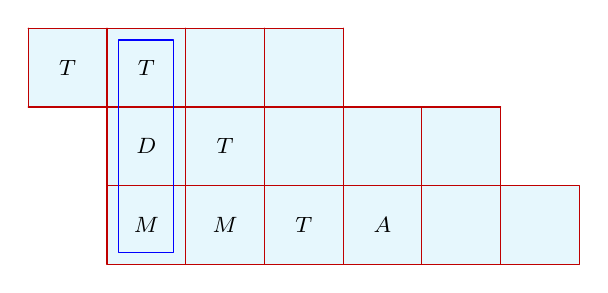
\begin{tikzpicture}[scale=1,font=\footnotesize, line join=round, line cap=round, >=stealth]
			\fill[cyan!10]
			(0,2) rectangle (4,3)
			(1,1) rectangle (6,2)
			(1,0) rectangle (7,1);
			\draw[red!75!black]
			(1,0) -- (7,0)
			(1,1) -- (7,1)
			(0,2) -- (6,2)
			(0,3) -- (4,3)
			(0,2) -- (0,3)
			(1,0) -- (1,3)
			(2,0) -- (2,3)
			(3,0) -- (3,3)
			(4,0) -- (4,3)
			(5,0) -- (5,2)
			(6,0) -- (6,2)
			(7,0) -- (7,1);
			\foreach \x/\y/\t in {
				0/2/T,1/2/T,
				1/1/D,2/1/T,
				1/0/M,2/0/M,3/0/T,4/0/A}
			{
				\node at (\x+0.5,\y+0.5) {$\t$};
			}
			\draw[blue] (1.15,0.15) rectangle (1.85,2.85);
		\end{tikzpicture}
	}
	\par
	\shortans[0]{330}
	\loigiai{
		Gọi các hàng từ trên xuống dưới lần lượt là $h_1$, $h_2$, $h_3$ với số lượng ô tương ứng là $4, 5, 6$.\\
		Số phần tử của không gian mẫu (xếp $8$ kí tự vào $15$ ô trống, trong đó có $4$ chữ $T$ giống nhau và $2$ chữ $M$ giống nhau) là:
		\[ n(\Omega) = \dfrac{\mathrm{A}_{15}^8}{4! \cdot 2!} = 5\,405\,400. \]
		\textbf{Bước 1:} Đếm số cách xếp xuất hiện chữ \textbf{TDM} (tạm thời bỏ qua điều kiện không có hàng trống). Gọi số cách này là $n_1$.
		\begin{itemize}
			\item Gọi $X$ là tập các cách xếp có chữ \textbf{TDM} trên một hàng.\\
			Số vị trí có thể đặt \textbf{TDM} trên các hàng $h_1, h_2, h_3$ lần lượt là $2, 3, 4$. Có tổng cộng $9$ vị trí.\\
			Sau khi đặt \textbf{TDM}, ta xếp $5$ kí tự còn lại ($1$ chữ $A$, $1$ chữ $M$, $3$ chữ $T$) vào $12$ ô trống. Số cách xếp là $\dfrac{\mathrm{A}_{12}^5}{3!}$.\\
			Suy ra $n(X) = 9 \cdot \dfrac{\mathrm{A}_{12}^5}{3!} = 142\,560$.
			\item Gọi $Y$ là tập các cách xếp có chữ \textbf{TDM} trên một cột.\\
			Chỉ có $3$ cột có đủ $3$ ô xếp dọc (tương ứng với cột thứ 2, 3, 4 từ trái sang). Mỗi cột có $1$ vị trí đặt \textbf{TDM}. Có tổng cộng $3$ vị trí.\\
			Xếp $5$ kí tự còn lại vào $12$ ô trống có $\dfrac{\mathrm{A}_{12}^5}{3!}$ cách.\\
			Suy ra $n(Y) = 3 \cdot \dfrac{\mathrm{A}_{12}^5}{3!} = 47\,520$.
			\item Tập $X \cap Y$ là các cách xếp có chữ \textbf{TDM} vừa trên hàng vừa trên cột.\\
			Vì chỉ có đúng $1$ chữ $D$ nên hai cụm \textbf{TDM} này bắt buộc phải giao nhau tại chữ $D$. Dựa vào cấu trúc lưới, có đúng $2$ vị trí giao nhau tạo thành dấu thập hợp lệ.\\
			Khi đó lưới đã dùng $5$ ô. Ta xếp $3$ kí tự còn lại ($1$ chữ $A$, $2$ chữ $T$) vào $10$ ô trống. Số cách xếp là $\dfrac{\mathrm{A}_{10}^3}{2!}$.\\
			Suy ra $n(X \cap Y) = 2 \cdot \dfrac{\mathrm{A}_{10}^3}{2!} = 720$.
		\end{itemize}
		Theo nguyên lí bù trừ: $n_1 = n(X) + n(Y) - n(X \cap Y) = 142\,560 + 47\,520 - 720 = 189\,360$.\\
		\textbf{Bước 2:} Đếm số cách xếp xuất hiện chữ \textbf{TDM} mà \textbf{có ít nhất 1 hàng bị bỏ trống}. Gọi số cách này là $n_2$.\\
		Vì cần xếp $8$ kí tự nên tối đa chỉ có $1$ hàng bị trống (nếu $2$ hàng trống thì số ô còn lại nhiều nhất là $6 < 8$). Hơn nữa, nếu có $1$ hàng trống thì không thể tạo được \textbf{TDM} dọc trên cột. Do đó chữ \textbf{TDM} bắt buộc phải nằm ngang.
		\begin{itemize}
			\item \textbf{Trường hợp 1:} \textbf{TDM} nằm ở $h_1$ (có $2$ vị trí).
			\begin{itemize}
				\item Nếu $h_2$ trống: $5$ kí tự còn lại xếp vào $15 - 3 (\text{của \textbf{TDM}}) - 5 (h_2) = 7$ ô trống. Có $\dfrac{\mathrm{A}_7^5}{3!}$ cách.
				\item Nếu $h_3$ trống: $5$ kí tự còn lại xếp vào $15 - 3 - 6 (h_3) = 6$ ô trống. Có $\dfrac{\mathrm{A}_6^5}{3!}$ cách.
			\end{itemize}
			Số cách TH1 là: $2 \cdot \left(\dfrac{\mathrm{A}_7^5}{3!} + \dfrac{\mathrm{A}_6^5}{3!}\right) = 1\,080$.
			\item \textbf{Trường hợp 2:} \textbf{TDM} nằm ở $h_2$ (có $3$ vị trí).
			\begin{itemize}
				\item Nếu $h_1$ trống: $5$ kí tự còn lại xếp vào $15 - 3 - 4 = 8$ ô trống. Có $\dfrac{\mathrm{A}_8^5}{3!}$ cách.
				\item Nếu $h_3$ trống: $5$ kí tự còn lại xếp vào $15 - 3 - 6 = 6$ ô trống. Có $\dfrac{\mathrm{A}_6^5}{3!}$ cách.
			\end{itemize}
			Số cách TH2 là: $3 \cdot \left(\dfrac{\mathrm{A}_8^5}{3!} + \dfrac{\mathrm{A}_6^5}{3!}\right) = 3\,720$.
			\item \textbf{Trường hợp 3:} \textbf{TDM} nằm ở $h_3$ (có $4$ vị trí).
			\begin{itemize}
				\item Nếu $h_1$ trống: $5$ kí tự còn lại xếp vào $15 - 3 - 4 = 8$ ô trống. Có $\dfrac{\mathrm{A}_8^5}{3!}$ cách.
				\item Nếu $h_2$ trống: $5$ kí tự còn lại xếp vào $15 - 3 - 5 = 7$ ô trống. Có $\dfrac{\mathrm{A}_7^5}{3!}$ cách.
			\end{itemize}
			Số cách TH3 là: $4 \cdot \left(\dfrac{\mathrm{A}_8^5}{3!} + \dfrac{\mathrm{A}_7^5}{3!}\right) = 6\,160$.
		\end{itemize}
		Suy ra $n_2 = 1\,080 + 3\,720 + 6\,160 = 10\,960$.\\
		\textbf{Bước 3:} Gọi $A$ là biến cố thỏa mãn yêu cầu bài toán.\\
		Số kết quả thuận lợi là $n(A) = n_1 - n_2 = 189\,360 - 10\,960 = 178\,400$.\\
		Xác suất $p = \dfrac{n(A)}{n(\Omega)} = \dfrac{178\,400}{5\,405\,400} = \dfrac{892}{27\,027}$.\\
		Vậy $10\,000p = 10\,000 \cdot \dfrac{892}{27\,027} \approx 330{,}04 \approx 330$.
	}
\end{ex}
\Closesolutionfile{ans}
\newpage
\indapan{12}{ans/ansTN-Dung}
\indapan[TF]{2}{ans/ansTN-DungSai}
\indapan[SA]{6}{ans/ansTN-DienKhuyet}
%%%%%%%%%%%%%%
%%nhãn kết thúc đề (để đếm số trang tự động mỗi đề)
\label{B\thedeso}